%\setcounter{chapter}{0}
%\setcounter{secnumdepth}{-1}

\chapter{Introduction and Motivation}\label{sec:intro}
The goal of this analysis is to provide insight into the mechanisms, baryon resonances and productions channels involved in \piz production for incident beam energies already explored as well as for incident beam energies in which there exists only a sparse and in some cases no amount of data.
Nucleons are composite particles, meaning they are made up of smaller constituents. To gain insight into the structure of the nucleon, physics employ baryon spectroscopy to explore for baryon resonances. Experimental, theoretical and phenomenological methods have been developed to refine and expand the known resonance masses, widths, and electromagnetic couplings~\cite{Dugger07}. Precise measurements of the cross-section and polarization asymmetries are important to extract photo-decay amplitudes and production mechanisms. Recently there has been improvement in Wide Angle Compton Scattering predictions using a General Parton Distribution (\abbr{GPD}) handbag model. This framework has also been recently adopted into \piz production~\cite{Huang2000} to describe the production as single quark excitation in photon-quark scattering.
%of   in which the production of the nucleons is considered in a 2 part soft and hard mechanism exchange.

In this analysis, we report on an experiment that was performed with the Cebaf Large Angle Spectrometer (\abbr{CLAS}) setup at the Thomas Jefferson National Accelerator Facility (\abbr{TJNAF}). The experiment used a tagged photon beam produced via bremsstrahlung from a 5.715~GeV electron beam delivered from the CEBAF accelerator. The photon beam struck a liquid hydrogen target. The reaction of interest is photoproduction of neutral pions on a hydrogen target, $\gamma p\to p\pi^0$, with subsequent Dalitz decay $\pi^0\to e^+e^-\gamma$ or standard decay plus photon conversion conversion mode $\pi^0\to \gamma\gamma\to e^+e^-\gamma$ . Neither the Dalitz decay mode of $\pi^0$ with very small branching ratio of $\sim 1.2\%$, nor the conversion mode from the main decay mode $\pi^0\to \gamma\gamma$ with branching ratio $\sim 98.8\%$ is preferred. The conversion rate of $\gamma$ to $e^+e^-$ is substantial enough that the Dalitz and the conversion process share the total statistical sample. The cross-section measurement is performed for the reaction $\gamma p\to pe^+e^-(\gamma)$ using a tagged photon beam spanning the energy interval  $E_{\gamma}=1.142$~GeV$-5.425$~GeV. In the final state of the reaction the photon is missing, $p e^+e^-$ are detected and $\pi^0$ is identified in the missing mass of the proton.

Using \epem decay products of \piz, contrary to $\gamma\gamma$ decay of \piz, along with detection of the proton allowed the experiment to run with high current. This was achieved by requiring a trigger configuration comprised of multiple charged tracks along with Cherenkov and Electromagnetic Calorimeter detection for photon beam energies $1.142$~GeV$ < E_{\gamma} < 3.6$~GeV. For photon beam energies greater than $3.6$~GeV a trigger configuration comprised of just multiple charged tracks was utilized.
\FloatBarrier
%
%
%
%
%. First we wanted to study $M_{e+e-}$ dependence of $\pi^0$ cross section, secondly and most importantly in the Dalitz decay mode final state contains three charged tracks, contrary to $\gamma\gamma$ decay, which allows to run experiment with high current, which otherwise wouldn't have been possible with single prong charged track, due to trigger and data acquisition limitations.
%\setcounter{secnumdepth}{2}
\section{Hadrons}
In the quark model, a hadron is a colorless particle formed of quarks and anti-quarks that are bound together by the strong force. Hadrons are organized and classified according to their quark content. The standard model permits multiple valence quark configurations for hadrons, however to date only two configurations have been verified, baryons and mesons. Baryons are hadrons with three quarks with suitable colors, while hadrons with two valence quarks, a quark and an anti-quark with color and ``anti-color'', are called mesons. Since baryons have an odd number of valence quarks, they are spin $\frac{1}{2}$ particles and thus are fermions, however mesons are spin 0 or 1 particles are bosons. As in any quantum-mechanical bound system, the valence quarks have a discrete energy level spectrum due to the various modes of the di-quark excitations, vibrations, orientations and vibrations which give rise to the quantum numbers $J^{PC}$. Here $J=L+S$ is defined as the total angular momentum containing orbital angular momentum $L$ and spin $S$, while $P=(-1)^{L+1}$ and $C= (-1)^{L+S}$ are defined as parity and charge conjugation.
% 
%The valence quarks in hadrons produce the quantum numbers $J^{PC}$, where $J=L+S$ is the total angular momentum created by the orbital angular momentum, L,  and the spin, S, of the particle. The ``P" stands for parity, $P = (-1)^{L+1}$, and ``C" is the charge conjugation, $C = (-1)^{L+S}$. Each type of meson can be categorized by their spin configuration and are shown in table 1 below.
% 
% 
%In the quark model, mesons are comprised of two valence quarks which are a quark and an anti-quark with color and ``anti-color''. Since mesons are comprised of a quark-antiquark pair, they are bosons. 
%These various modes give rise to the quantum numbers of the mesons via their flavor and symmetry $J^{PC}$.
%The different mesons can be classified into types according to their spin configurations. 
Each type of meson can be categorized by their spin configuration and are shown in Tab.~\ref{tab:meson_type}.
\begin{table}
\begin{minipage}{\textwidth}
\begin{center}
\begin{singlespacing}

\caption[Types of mesons]{\label{tab:meson_type}Types of mesons}

\begin{tabular}{c c c c c c} % centered columns (4 columns)
\hline%inserts double horizontal lines
Type & J & P & L & S & J$^{P}$ \\ [0.5ex] % inserts table
%heading
\hline % inserts single horizontal line
Pseudoscalar & 0 & - & 0 & 0 & 0$^-$\\
Scalar & 0 & + & 1 & 1 & 0$^+$\\
Vector & 1 & - & 0 & 1 & 1$^-$\\
Axial Vector & 1 & + & 1 & 0 & 1$^+$\\
Tensor & 2 & + & 1 & 1 & 2$^+$ \\ [1ex]
\hline \hline%inserts single line
\end{tabular}

\end{singlespacing}
\end{center}
\end{minipage}
\end{table}
\vspace{20pt}


%\begin{tabular}{c||c|c|c|c||c}
%Type & $S$ & $L$ & $P$ & $J$ & $J^P$ \\ \hline \hline
%Pseudoscalar meson & 0 & 0 & - & 0 & $0^-$\\ \hline 
%Axial vector meson & 0 & 1 & + & 1 & $1^+$\\ \hline 
%Vector meson & 1 & 0 & - & 1 & $1^-$\\ \hline 
%Scalar meson & 1 & 1 & + & 0 & $0^+$\\ \hline 
%Tensor meson & 1 & 1 & + & 2 & $2^+$
%
%
%\end{tabular}
\FloatBarrier

\subsection{Light Pseudoscalar Mesons} 
The following analysis will concentrate on the lightest neutral pseudoscalar meson, $\pi^0$, which is member of the family of $P_p$($\pi^{0}, \eta, \eta'$)($J^{P}=0^{-}$) mesons that are subject to U(3) flavor symmetry. The nonet, the resulting nine states that can be decomposed into a singlet and an octet state, of the pseudoscalar mesons are seen in Fig.~\ref{fig:nonet.pseud}, where strangeness increases upward on the page and charge increases toward the right side of the page.
\begin{figure}[h!]\begin{center}
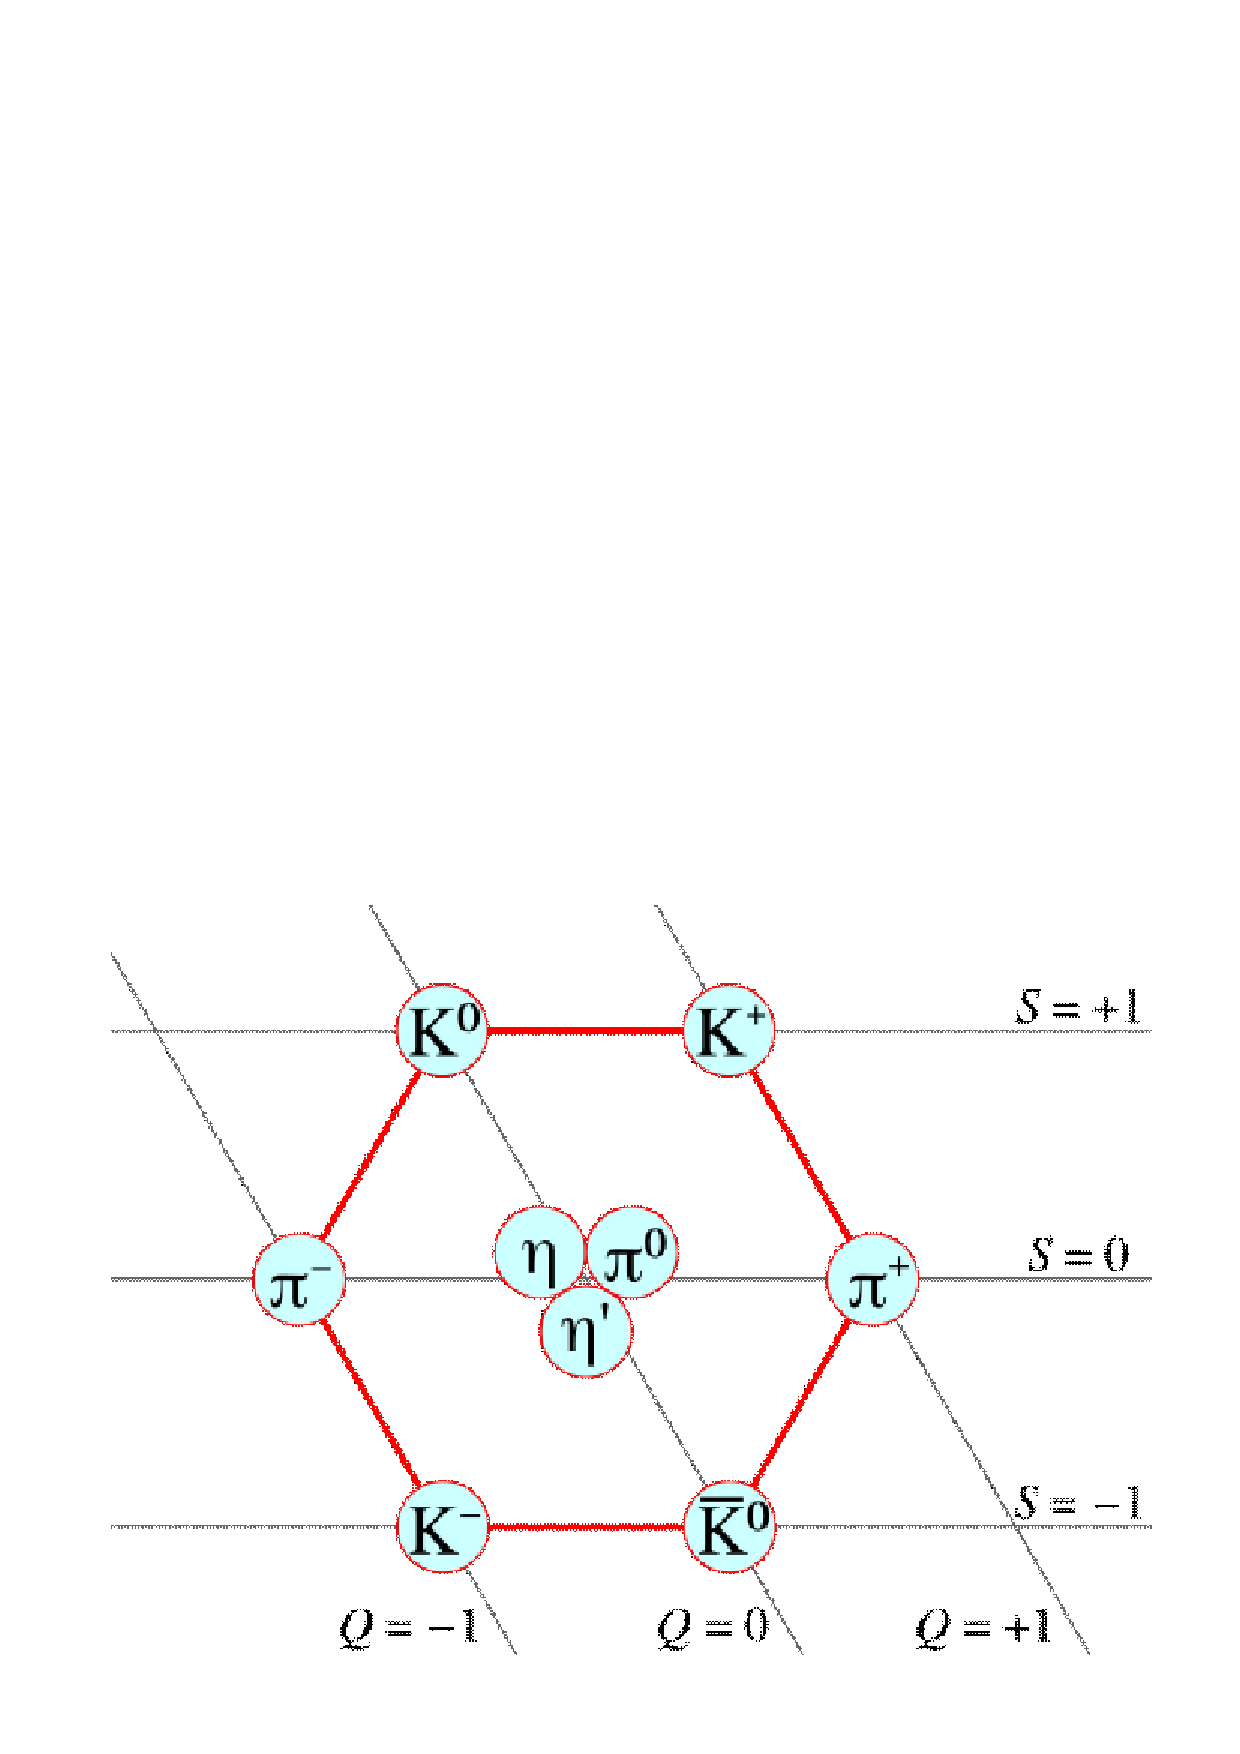
\includegraphics[width= 0.8 \figwidth ,height=\qfigheight]{\grpath/intro/pseudoscalar.pdf}
\caption[Nonet of Pseudoscalar Mesons]{\label{fig:nonet.pseud}Nonet of Pseudoscalar Mesons~\cite{wiki1}.}
\end{center}\end{figure}
It should be noted that the $\eta$ and $\eta'$ are not exact octet ($\eta_{8}$) and singlet ($\eta_{0}$) states, as they are linear combinations of $\eta_{8}$ and $\eta_{0}$ according to:
\begin{eqnarray}
\left(
\begin{array}{cc}
\eta \\
\eta ' 
\end{array}
\right)
& = &
\left(
\begin{array}{cc}
-\sin\theta_{mix} & \cos\theta_{mix} \\
\cos\theta_{mix} & \sin\theta_{mix}
\end{array}
\right)
\cdot
\left(
\begin{array}{cc}
\eta_{0} \\
\eta_{8}
\end{array}
\right)
\end{eqnarray}
where $\theta_{mix} = -18.6^{\circ}$\cite{Goity} and $\eta_{8}$ and $\eta_{0}$  have quark content of:
\begin{eqnarray}
\eta_{0} &\rightarrow & \sqrt{\frac{1}{6}}(u\overline{u} + d\overline{d} +  s\overline{s})\nonumber\\
\nonumber \\
\eta_{8} &\rightarrow & \sqrt{\frac{2}{3}}(u\overline{u} + d\overline{d} - 2s\overline{s})\nonumber \\
\nonumber \\
\nonumber 
\end{eqnarray}
The physical masses of $\eta$ and $\eta'$ are $m_{\eta} = 547.51\pm 0.18$~MeV \cite{pdg2014}, $m_{\eta'} =957.78 \pm 0.14$~MeV \cite{pdg2014}, and the widths are $\Gamma_{\eta} =1.30\pm0.07$~keV and $\Gamma_{\eta'} = 0.203\pm0.016$~MeV.
The lightest of the mesons $\pi^{0}$ has a quark content of:
\begin{eqnarray}
\pi^{0} = \frac{1}{\sqrt{2}}(u\overline{u} - d\overline{d})\nonumber
\end{eqnarray}
and mass of $m_{\pi^{0}} = 134.9766 \pm 0.0006$~MeV \cite{pdg2014}. The decay modes for \piz are given in Table \ref{tab:pi0}.
\begin{table}
\begin{minipage}{\textwidth}
\begin{center}
\begin{singlespacing}

\caption[Branching Ratios of the \piz Decay]{\label{tab:pi0} Branching ratios of the \piz decay.~\cite{pdg2014}}
\begin{tabular}{l|c}
\hline												
Mode	& Branching ratio \\ \hline 	
$\pi^0 \to 2\gamma$	 &   $ (98.823 \pm 0.034)  \cdot 10^{-2}$ \\	
$\pi^0 \to e^+ e^-\gamma$  &  $  (1.174 \pm 0.035)  \cdot 10^{-2}$ \\
$\pi^0 \to \gamma $ positronium   &  $ (1.82 \pm 0.29)  \cdot 10^{-9}$\\
$\pi^0 \to  e^+ e^+ e^- e^-	$  &  $( 3.34 \pm 0.16)  \cdot 10^{-5}$\\
$\pi^0 \to  e^+ e^-$  &  $ (6.46 \pm 0.33)  \cdot  10^{-8}$\\
$\pi^0 \to 4\gamma$	&  $<2 \cdot 10^{-8}$\\
$\pi^0 \to \nu \bar \nu$  &  $<2.7 \cdot 10^{-7}$\\
$\pi^0 \to \nu_e \bar \nu_e$  &  $<1.7 \cdot 10^{-6}$\\
$\pi^0 \to \nu_{\mu} \bar \nu_{\mu}$  &  $<1.6 \cdot 10^{-6}$\\
$\pi^0 \to \nu_\tau \bar \nu_\tau $  &  $<2.1 \cdot 10^{-6}$\\
$\pi^0 \to \gamma \nu \bar \nu$	 &  $<6 \cdot 10{-4}$\\
\hline \hline%inserts single line
\end{tabular}

\end{singlespacing}
\end{center}
\end{minipage}
\end{table}
\vspace{20pt}

%\begin{figure}[h!]\begin{center}
%\subfloat[Nonet of Pseudoscalar Mesons][]{ %Feynman diagram of \piz two photon decay
%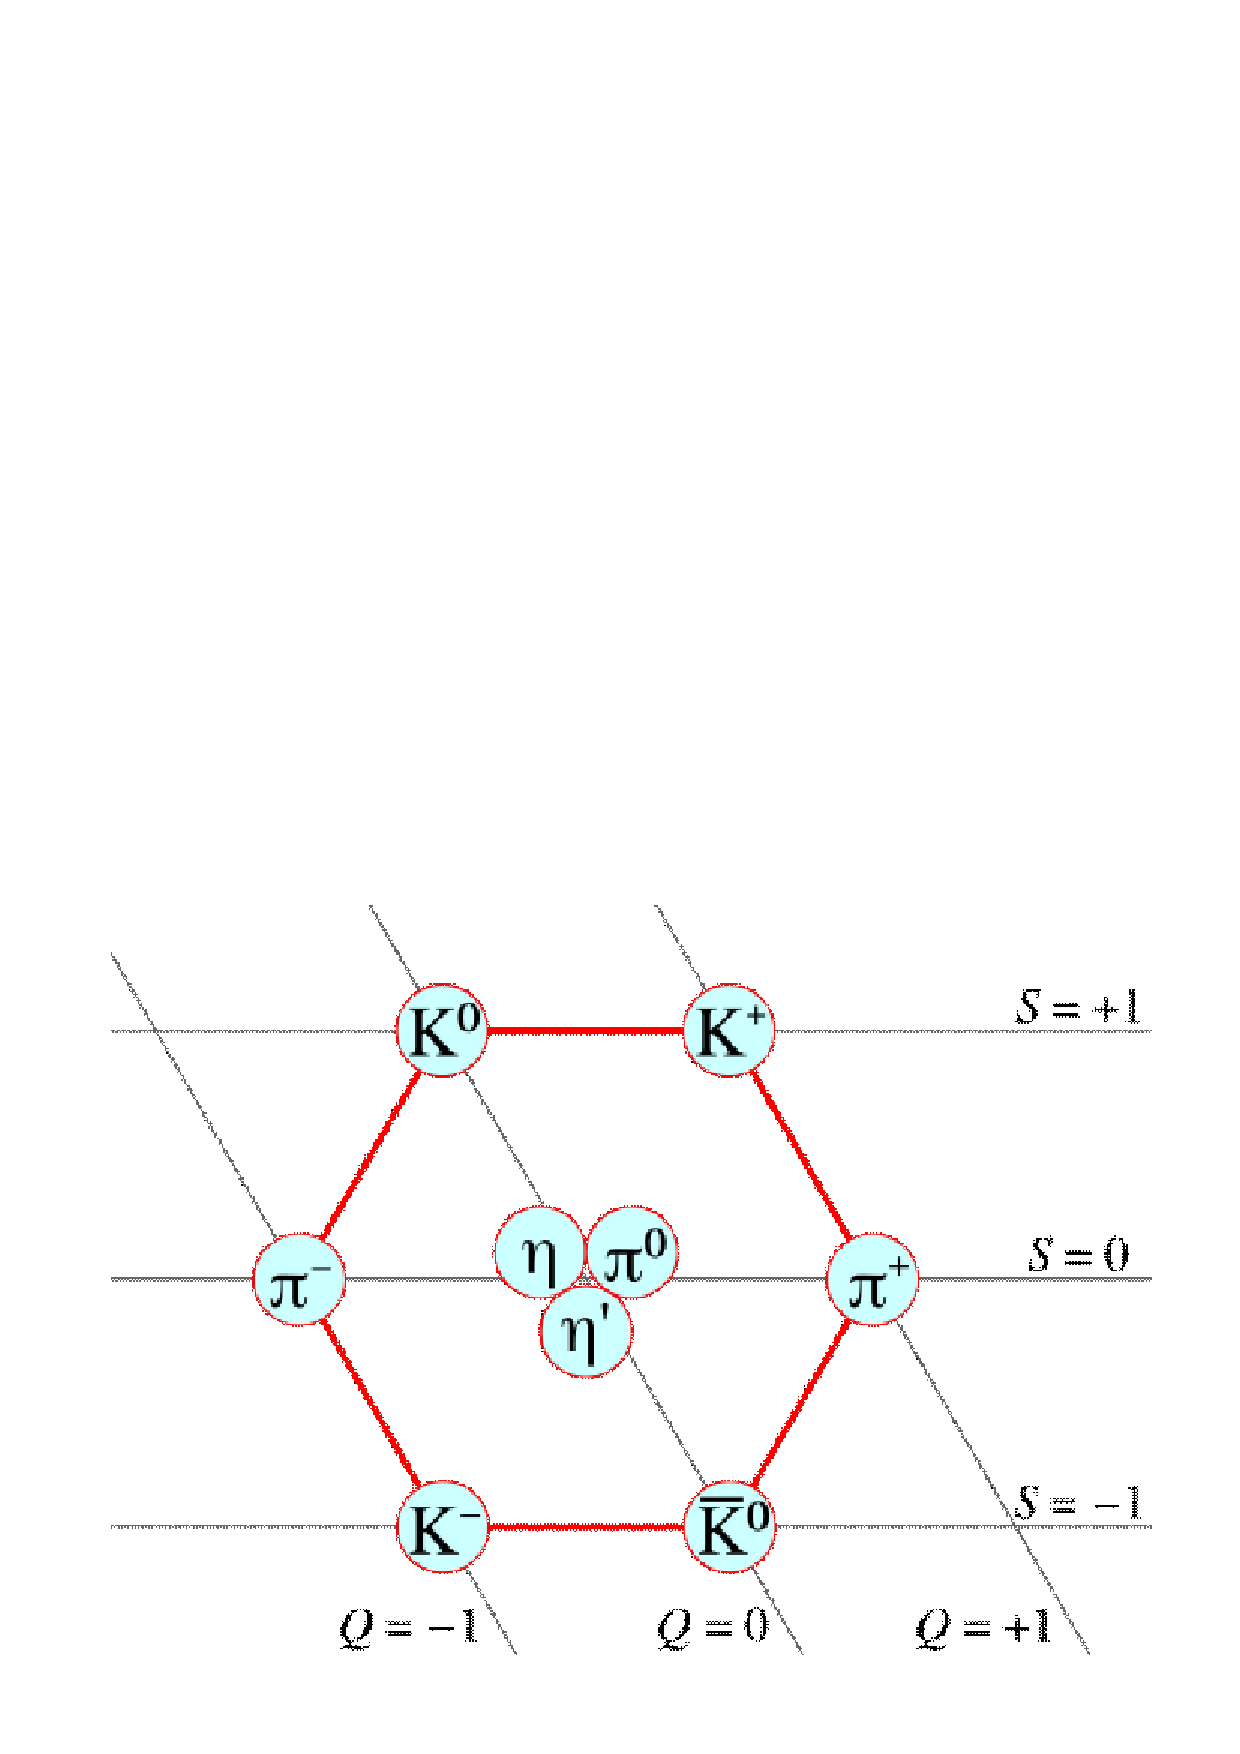
\includegraphics[width=0.65\columnwidth,height=0.5\qfigheight]{\grpath/intro/pseudoscalar.pdf}\label{fig:nonet.pseud}
%}
%
%\subfloat[Nonet of Vector Mesons][]{ %Feynman diagram of \piz Dalitz decay
%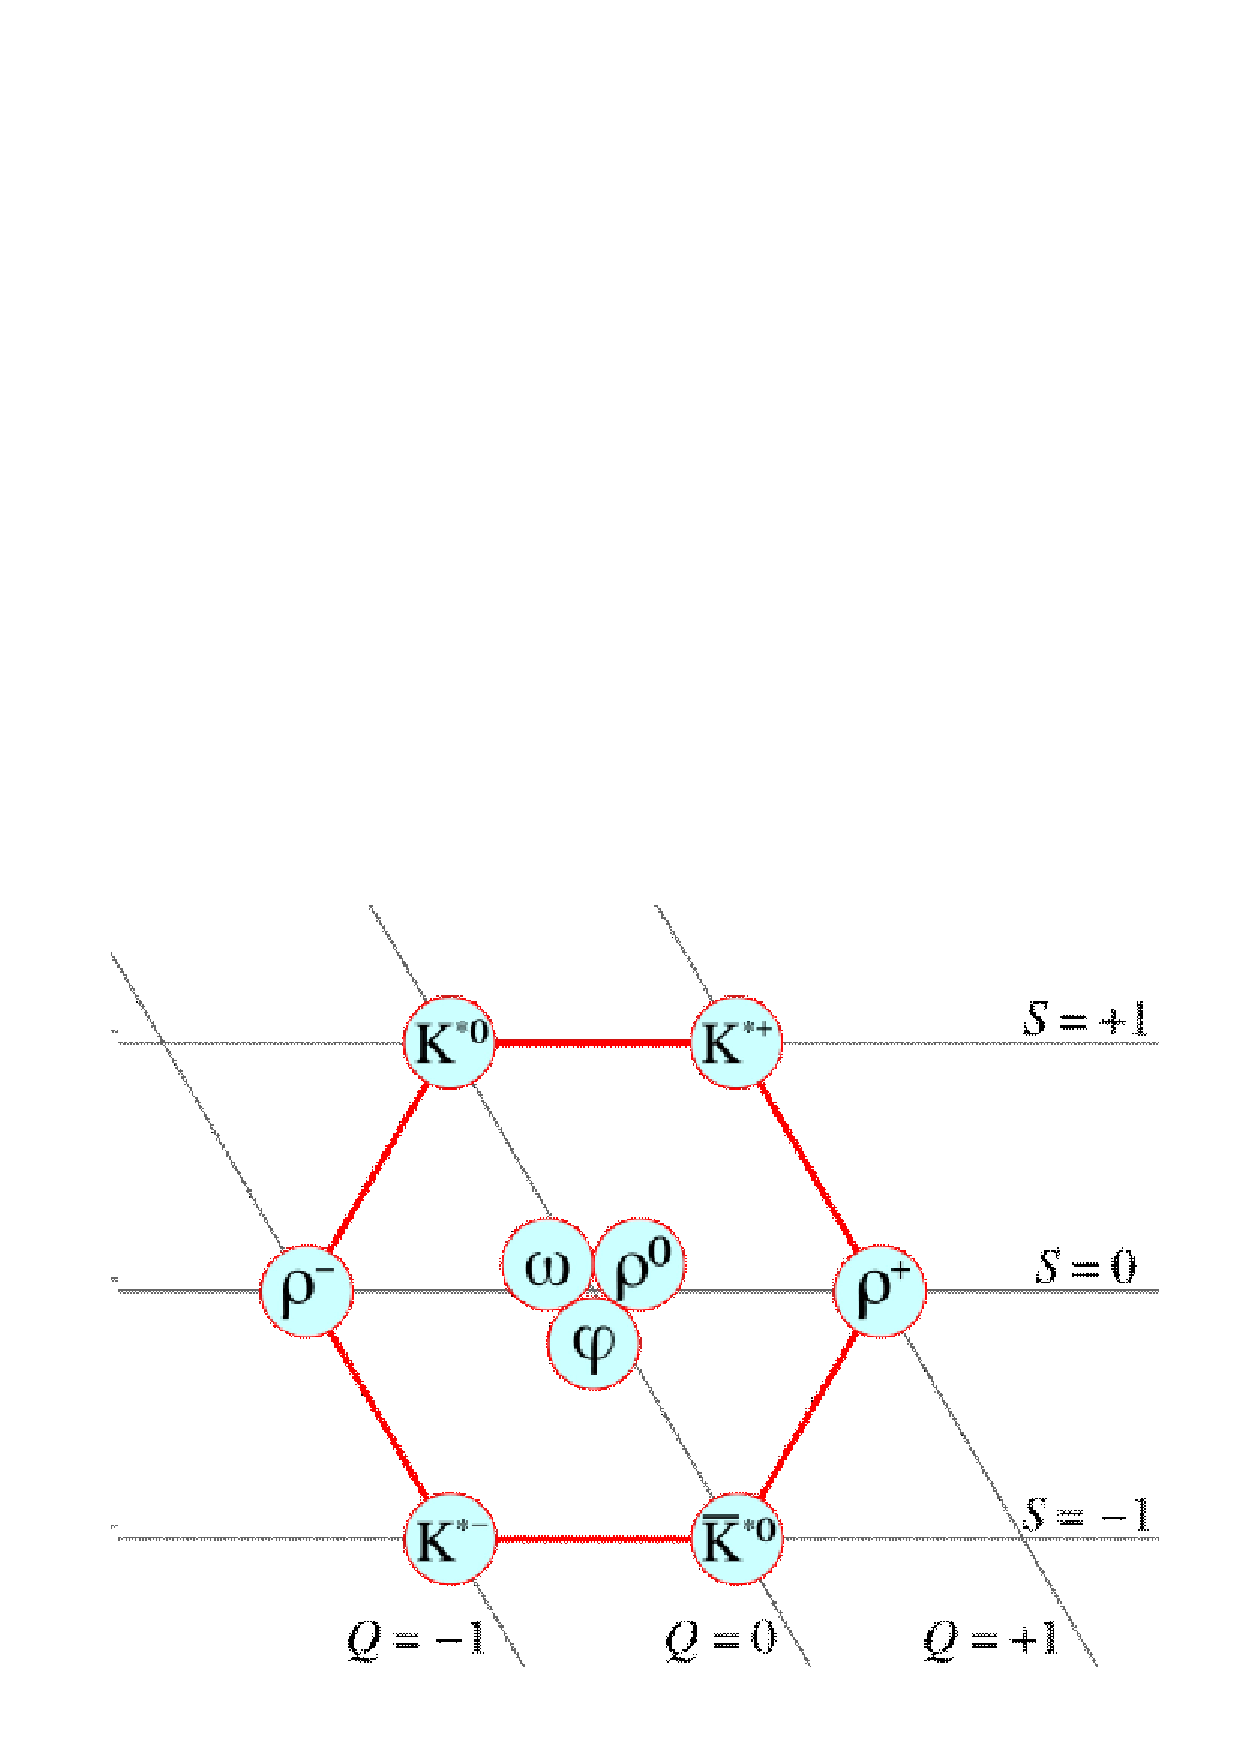
\includegraphics[width=0.65\columnwidth,height=0.5\qfigheight]{\grpath/intro/vector.pdf}\label{fig:nonet.vect}
%}
%\caption[Nonet of Pseudoscalar and Vector Mesons]{\label{fig:piz.alldecay}Nonet of pseudoscalar mesons~\subref{fig:nonet.pseud}. Nonet of vector mesons~\subref{fig:nonet.vect}.}
%
%\end{center}\end{figure}
%
%The \piz is the lightest meson with a mass of $m_{\pi^0}= (134.9766 \pm 0.0006) {\rm MeV}$ \cite{pdg2014}. The quark content is:
%\begin{equation}
% \pi^0 : \frac{1}{\sqrt{2}}\left(u \bar u  - d \bar d \right).
%\end{equation}

%In the intended analysis, it is planned to investigate the cross-section of the \piz.

\section{\piz Production} \label{sec:into:xsection}
The present analysis uses two approaches to describe the behavior of the \piz cross-section. One approach is for incident photon beam energies less than 2.8~GeV where the missing resonance search is most valid and the data can be described well by coupling of the \piz electromagnetic wave functions. The second approach attempts to describe the behavior of the \piz by using General Parton Distribution models, \abbr{GPD} for incident photon beam energies greater than 2.8~GeV.
%The physics behind this is that since the photon couples to charged-fermion pairs, a part of its cross-section could be described by considering interactions between the hadron and a virtual fermion pair~\cite{butterworth}.


\subsection{Low Energy \piz Production}\label{sec:into:xsection.low}

\begin{figure}[h!]\begin{center}
\includegraphics[width=0.5 \figwidth,height= \qfigheight]{\figures/feyman_pi0IV.pdf}
\caption[Diagram for photoproduction of the \piz meson]{\label{fig:xsection.pi0feynman}	Diagram for photoproduction of the \piz meson. $k$ and $p_i$ are the incident photon beam and target proton 4-moment respectively, $q$ and $p_f$ represent the produced \piz meson and scattered proton 4-momenta respectively.}
\end{center}\end{figure}
For incoming photon beam energies less than 2.8~GeV, the production of the \piz meson, with 4-momenta $q$, in photon-proton reactions, with 4-momenta $k$ and $p_i$ respectively and $p_f$ being the 4-momenta of the scattered proton (see Fig.~\ref{fig:xsection.pi0feynman}),  can be described in terms of the three Lorentz invariant Mandelstam variables, $s$, $t$ and $u$, where
\begin{align}
s = (k+p_i)^2 = (q+p_f)^2 \nonumber \\
t=(p_i-p_f)^2 = (k-q)^2  \nonumber \\
u = (k - p_f)^2 = (p_i-q)^2 \ .
\end{align}
The sum of the Mandelstam variables linearly combine to give the sum of masses of the particles involved:
\begin{align}
s + t + u = \sum\limits_{i}^{4} m_i^2 
\end{align}
and the definition of Lorentz-invariant mass:
\begin{align}
p_i\cdot p_i = E_i^2 - \mathbf{p_i}\cdot \mathbf{p_i} = m_i^2 \ .
\end{align}
Using energy-momentum conservation:
\begin{align}
k + p_i = q+p_f \,
\end{align}
it is seen that only three of the four momenta are independent. Conventionally the use of $k$ and $q$ and a combined 4-momenta of the nuclei 
\begin{align}
P = \frac{1}{2}(p_i+p_f)
\end{align}
are used as the independent kinematic variables. The three Mandelstam variables can be express in terms of the other two, therefore the scattering process is described by functions of only two of the Mandelstam variables. Conventionally they are chosen to be $s$ and $t$, which in the center-of-mass frame (C.M.) of the initial and final state equal the invariant mass squared of the system and the momentum transfer in the production process respectively.
\subsection{Isospin Representation}\label{sec:isospin}
The scattering matrix $\mathcal{M}$ for single pion photoproduction process is written as:
\begin{align}
\mathcal{M} =  (\epsilon_\mu k_\nu - \epsilon_\nu k_\mu)&[ \frac{1}{2}i \gamma_5 \gamma_\mu \gamma_\nu A_1(s,t) + 2 i \gamma_5 P_\mu(q-\frac{1}{2}k)_\nu A_2(s,t) \nonumber \\ & + \gamma_5 \gamma_\mu q_\nu A_3(s,t) + \gamma_5 \gamma_\mu(2P_\nu- i M\gamma_\nu) A_4(s,t) ] \ ,
\end{align}
where $M$ is the nucleon mass, $\epsilon$ is the photon polarization and $A_i(s,t)$ are the invariant functions of the Mandelstam invariants $s$ and $t$. The amplitude $A_i(s,t)$ refers to the emission of a pion of isospin index $\alpha$, and is given by the well-known formula:
\begin{align}\label{eq:isoscal_vec}
A_i(s,t)= A_i^{(0)}\tau_\alpha + A_i^{(+)}\delta_{\alpha 0} + \frac{1}{2} A_i^{(-)}\left[\tau_\alpha,\tau_0\right] \ ,
\end{align}
where $\tau_\alpha$ are the nucleon isospin transition operators, where the sign of $\alpha$ indicates the opposite sign of the pion isospin, this is by convention. Eq.~\ref{eq:isoscal_vec} assumes that the photon interaction with hadrons occurs through isoscalar and isovector parts, so that $A_i^{(0)}$ is the isoscalar amplitude that corresponds to a zero net isospin transistion resulting from the electromagnetic field. The amplitudes $A_i^{(+)}$ and $A_i^{(-)}$ are the isovector amplitudes and can be combined as $A_i^{(+)} + 2 A_i^{(-)}$ and $A_i^{(+)} - A_i^{(-)}$ so that the pion nucleon final state has definite isospin $\frac{1}{2}$ and $\frac{3}{2}$ respectively~\cite{Rosenfeld} by use of
\begin{align}
A^S = -(3)^\frac{1}{2}A^{(0)} \nonumber \\
A^{V1} = \left(\frac{1}{3}\right)^\frac{1}{2}A_i^{(+)} + 2 A_i^{(-)} \nonumber \\
A^{V2} = \left(\frac{2}{3}\right)^\frac{1}{2}A_i^{(+)} - A_i^{(-)} \ ,
\end{align}
where $A^S$, $A^{V1}$ and $A^{V2}$ are the isoscalar amplitude, isovector amplitude of isospin $\frac{1}{2}$ and isovector amplitude of isospin $\frac{3}{2}$ respectively.
The four possible pion nucleon amplitudes $A_i(s,t)$ of the initial and final state particles in the pion photoproduction process are in terms of the isoscalar and isovector are:
\begin{align}
A_1(\gamma p \to n \pi^+) = -\sqrt{\frac{1}{3}}A^{V3} + \sqrt{\frac{2}{3}}(A^{V1} - A^{S}),\\
A_2(\gamma p \to p \pi^0) = \sqrt{\frac{2}{3}} A^{V3} + \sqrt{\frac{1}{3}}(A^{V1}-A^{S}),\\
A_3(\gamma n \to p \pi^-) = \sqrt{\frac{1}{3}}A^{V3} - \sqrt{\frac{2}{3}}(A^{V1} + A^{S}),\\
A_3(\gamma n \to n \pi^0) = \sqrt{\frac{2}{3}}A^{V3} + \sqrt{\frac{1}{3}}(A^{V1} + A^{S}).
\end{align}
Since the combination $\sqrt{\frac{2}{3}}(A^{V1} \mp A^{S})$ gives the coupling of photons to positive and neutral isospin-$\frac{1}{2}$ states, respectively, ~\protect\cite{Rosenfeld}, defined explicitly
%
\begin{align}
&&A^p = + \sqrt{\frac{2}{3}}(A^{V1} - A^{S}),\\
&&A^n = -\sqrt{\frac{2}{3}}(A^{V1} + A^{S}).
\end{align}
\subsection{Structure Functions}\label{sec:CGLN}
To obtain the scattering matrix elements in terms of experimental quantities, it is preferred and easier to work in the C.M. system and reduce the $\mathcal{M}$ to a form $\mathcal{F}$ by equating the invariant form of the scattering matrix elements in each frame, i.e.:
\begin{align}
\bar{u}(p_2)\mathcal{M} u(p_1) \equiv \frac{4 \pi W}{M}\chi_f^\dagger \mathcal{F} \chi_i \ ,
\end{align}
where $\bar{u}(p_2)$ and $u(p_1)$ are final and initial state Dirac spinors respectively and $\chi_f$ and $\chi_i$ are final and initial state Pauli spinors. The differential cross-section for single pion production is:
\begin{align}
\frac{d\sigma}{d\Omega} = \frac{q}{k}| \bra{f}\mathcal F \ket{i}|^2,
\end{align}
The expression to express Dirac spinors in terms of Pauli spinors is written as:
\begin{align}
\mathcal{F} = & i\vec{\mathbf{\sigma}}\cdot \vec{\mathbf{\epsilon}} \mathcal{F}_1 + \frac{1}{qk}(\vec{\mathbf{\sigma}}\cdot \vec{\mathbf{q}})\vec{\mathbf{\sigma}} \cdot(\vec{\mathbf{k}}\times \vec{\mathbf{\epsilon}}) \mathcal{F}_2 \nonumber \\ & + \frac{i}{qk}(\vec{\mathbf{\sigma}}\cdot \vec{\mathbf{k}})(\vec{\mathbf{q}}\cdot \vec{\mathbf{\epsilon}})\mathcal{F}_3 + \frac{i}{q^2}(\vec{\mathbf{\sigma}}\cdot \vec{\mathbf{q}})(\vec{\mathbf{q}}\cdot \vec{\mathbf{\epsilon}})\mathcal{F}_4 \ ,
\end{align}
where $\vec{\mathbf{k}}$ and $\vec{\mathbf{q}}$ are the C.M. 3-momenta and $\vec{\mathbf{\epsilon}}$ is the polarization of the photon. The relationship between $A_i$ and $\mathcal{F}$ is found using the relations:
\begin{align}
\mathcal{F}_1 = \frac{W- M}{8 \pi W }(D_1 D_2)^{\frac{1}{2}}\left[ A_1+(W-M)A_4 - \frac{k_0q_0-\vec{\mathbf{k}}\cdot \vec{\mathbf{q}}}{W-M}(A_3-A_4)\right] \\
\mathcal{F}_2 = qk \frac{W- M}{8 \pi W }(\frac{D_2}{D_1})^{\frac{1}{2}}\left[ -A_1+(W+M)A_4 + \frac{k_0q_0-\vec{\mathbf{k}}\cdot \vec{\mathbf{q}}}{W+M}(A_3-A_4)\right]  \\
\mathcal{F}_3 =qk \frac{W- M}{8 \pi W }(D_1 D_2)^{\frac{1}{2}}q\left[(W-M)A_2 + A_3 - A_4\right]\\
\mathcal{F}_4 = q^2 \frac{W- M}{8 \pi W }(\frac{D_2}{D_1})^{\frac{1}{2}}q\left[ -(W+M)A_2 + A_3 - A_4\right] 
\end{align}
where
\begin{align}
D_1 = (M^2 + \vec{\mathbf{k}}^2)^{\frac{1}{2}}+M \\
D_2 = (M^2 + \vec{\mathbf{q}}^2)^{\frac{1}{2}}+M \ .
\end{align}
$\mathcal{F}_i(s,t)$ are known as structure functions, alternatively known by Chew, Goldberger, Low and Nambu (\abbr{CGLN}) amplitudes. These amplitudes describe photoproduction as a function of $s$ and $t$, and therefore in terms of momentum transfer. To represent the process in terms of angular momentum transitions, expansion of the structure functions as partial waves in derivatives of Legendre polynomials, $P_l^\prime(\cos\theta)$, results in the four multipole series:
\begin{align}
&&\mathcal{F_1} = \displaystyle\sum_{l=0}^{\infty}[lM_{l+} + E_{l^+}]P_{l+1}^{\prime}(\cos\theta) + [(l+1)M_{l-1} + E_{l-}]P_{l-1}^{\prime}(\cos\theta)\\
&&\mathcal{F_2} = \displaystyle\sum_{l=1}^{\infty}[(l+1)M_{l+}+lM_{l-}]P_{l}^{\prime}(\cos\theta)\\
&&\mathcal{F_3} = \displaystyle\sum_{l=1}^{\infty}[E_{l+}-M_{l+}]P_{l+1}^{\prime \prime}(\cos\theta) + [E_{l-} + M_{l-}]P_{l-1}^{\prime \prime}(\cos\theta)\\
&&\mathcal{F_4} = \displaystyle\sum_{l=1}^{\infty}[M_{l+} - E_{l+} - M_{l-} - E_{l-}]P_{l}^{\prime \prime}(\cos\theta)
\end{align}
The energy-dependent amplitudes $M_{l\pm}$ and $E_{l\pm}$ refer to transitions initiated by magnetic and electric radiation, respectively, leading to final states of orbital angular momentum $l$ and total angular momentum $j=l\pm\frac{1}{2}$. 

The energy-dependent amplitudes $M_{l\pm}$ and $E_{l\pm}$ cannot be extracted directly from measurements, however using models on measured differential cross-sections and polarizations aide in the determination of the amplitudes. Constraining the production amplitudes aides in the determination of resonances. One such model that is used in this thesis is the SAID parameterization model discussed in Sec~\ref{sec:intro.said}. 


\subsection{SAID}\label{sec:intro.said}

SAID~\cite{SAID} is a repository of experimental data and an interactive analysis facility, allowing to compare and extract data and partial wave solutions (PWA) for a variety of photoproduction, electro-production and pion production reactions. It was created by R. A. Arndt and L. D. Roper for the use of verifying model calculations against measured/fitted data, compare model calculations against SAID predictions for unmeasured observables, experimental planning, and simulations and event generators.

SAID is based upon the theoretical framework given in~\ref{sec:isospin}. SAID generates resonance couplings, in terms of angular momentum and isospin quantum numbers, that are extracted from a fit-based determination of multipoles using both an energy-dependent and an energy-independent parametrization. The photoproduction amplitude is assumed to be in the form of a Breit-Wigner and a background term in the form of~\cite{ar90};
\begin{align}
A=A_l(1+iT_\pi)=A_r\left(\frac{k_0q_0}{kq}\right)^{\frac{1}{2}} \frac{W_0\sqrt{\Gamma \Gamma_{\gamma}}}{W_0^2-W^2-iW_0\Gamma} \ ,
\end{align}
in which $A_l$ is the background parameter, $W_0$, $\Gamma$ and $\Gamma_{\gamma}$ are functions of the full width $\Gamma_{0}$ and $A_R$ being the resonant parameter in the form of;
\begin{align}
A_r=\frac{\mu}{q}\left(\frac{k}{q}\right)^l\sum_{n=0}^{N}p_n\left(\frac{E_{\pi}}{\mu}\right)^n
\end{align}
where $k_0$ and $q_0$ are the pion and photon momenta at the resonance energy, $\mu$ is the pion mass, $E_{\pi}$ is the pion kinetic energy in the lab frame and $p_n$ is a free parameter. The background term is expanded as a set of Legendre polynomial terms with associated free parameters along with a sum of a pseudoscalar Born partial waves, which are determined by fitting the data. Multipoles can then be extracted by a fit of $A$ close to the resonance position.

\subsection{Summary}
A full set of differential cross-sections and polarization observables is required for the determination of multipoles. These can be related to the invariant amplitudes as functions of $W$ and $\cos\theta$. For the separation of the different isospin contributions, both the proton and the neutron pion-photoproduction measurements are needed. An understanding of the invariant amplitudes, and subsequent CGLN structure functions, can provide information on the multipole transitions taking place. This  allows to get direct information about the quantum numbers of the produced resonant states and constrain their position, widths and couplings.
The work of this thesis is devoted to measuring of the differential cross-sections for better fit determinations and possible resonance searches using the SAID parameterizations.
\subsection{High Energy \piz Production}\label{sec:into:xsection.high}
%ere is the citation ~\cite{key1, key2,Rad1996, Diehl}
The production of the \piz meson in photon-proton reactions, for incoming photon beam energies greater than 2.8~GeV, is considered to be a hard exclusive reaction. One approach to study the \piz production, in photon-proton reactions, is use the handbag model. In the handbag approach, the reaction is factorized into two parts. The first part is when one quark from the incoming and one from the outgoing nucleon participate in the hard sub-process, small blob in Fig.~\ref{fig:xsection.handbag}. This hard sub-process is achieved when the incident photon excites a quark, since quarks are bound quantum particles, the excited quark produces a jet of quarks that form the meson and then de-excites back into the nucleon. This is calculable using pQCD. The second part ,the soft part seen as the large blob in Fig.~\ref{fig:xsection.handbag} , consists of all the other quarks that are spectators and can be described in terms of GPDs~\cite{key1, key2,Rad1996, Diehl}. The hard exclusive meson (M) photo-production process factorizes into, $\gamma q \to Mq$, this is depicted in Fig.~\ref{fig:xsection.handbag}. The handbag mechanism is applicable when the Mandelstam variables, $s$, $t$, $u$, are large as compared to a hadronic scale of order 1 GeV . In Ref.~\cite{Huang2000} a model, derived from the handbag approach, has been applied to predict angular dependence of scaled photoproduction cross section of \piz and is illustrated in Fig.~\ref{fig:xsection.handbag.cal}. In the analysis presented, this model will investigated using the data obtained in \abbr{CLAS}.

\begin{figure}[h!]\begin{center}
\includegraphics[width= 0.8 \figwidth ,height=\qfigheight]{\grpath/intro/handbag.pdf}
\caption[The handbag-type diagram for photoproduction of mesons]{\label{fig:xsection.handbag}	The handbag-type diagram for photoproduction of mesons. The large blob represents a sum over all spectator configuration. $k_j$ and $k_j^{\prime}$  denote the momenta of the active partons. The small blob stands for meson photoproduction off partons.}
\end{center}\end{figure}

\begin{figure}[h!]\begin{center}
\includegraphics[width= 0.8 \figwidth ,height=\qfigheight]{\grpath/intro/photo-fig7.pdf}
\caption[The soft physics contribution to the cross-section for photoproduction of \piz]{\label{fig:xsection.handbag.cal}The soft physics contribution to the cross-section for photoproduction of \piz scaled by s$^7$ versus $\cos\theta$, where $\theta$ is the scattering angle in the $\gamma p$ c.m. system~\cite{Huang2000}.}
\end{center}\end{figure}
\FloatBarrier


% %
\section{\piz Decays}\label{sec:intro.decays}
The main decays studied for this analysis are when a pseudoscalar meson, $P_p$($\pi^{0}$, $\eta$, $\eta'$), decays via 2 photons $\gamma \gamma$ or a photon $\gamma$ and a dilepton ($l^{+}l^{-}$) pair, which are the two most prevalent decays of \piz as shown in Table~\ref{tab:pi0}. Figure~\ref{fig:piz.alldecay} illustrates the Feynman diagrams for the ``Two photon decay'' and the ``Dalitz decay''.
\begin{figure}[h!]\begin{center}
\subfloat[Feynman Diagram of \piz Two Photon Decay][]{ %Feynman diagram of \piz two photon decay
\includegraphics[width=0.65\columnwidth,height=0.5\qfigheight]{\grpath/intro/decays/P_to_gamgam_wnotation.pdf}\label{fig:piz.gamgam}
}

\subfloat[Feynman Diagram of \piz Dalitz Decay][]{ %Feynman diagram of \piz Dalitz decay
\includegraphics[width=0.65\columnwidth,height=0.5\qfigheight]{\grpath/intro/decays/P_to_lepsgam_wnotation.pdf}\label{fig:piz.dalitz}
}
\caption[Feynman diagram of $P_p$($\pi^0$) two photon decay and Dalitz decay]{\label{fig:piz.alldecay}Feynman diagram of $P_p$($\pi^0$) two photon decay~\subref{fig:piz.gamgam}, $\epsilon_1$ and $\epsilon_2$ are the polarizations, $p$ and $k$ are 4-momenta of the photons.  Feynman diagram of $P_p$($\pi^0$) Dalitz decay~\subref{fig:piz.dalitz}, the variable $s_\pm$ are the spin helicities of the outgoing leptons $l^\pm$ with 4-momenta $p_{\pm}$ and $\epsilon$ is the polarization of the outgoing photon with 4-momenta $k$. In both diagrams $\mathcal{M}$ is the form factor.}

\end{center}\end{figure}
\FloatBarrier
\subsection{Two Photon Decay}\label{sec:piz.gg}
As shown in Fig.~\ref{fig:piz.gamgam}, the two photon decay can be expressed in terms of the respective momentum, $P_p$($\pi^0$)$\to \gamma(\epsilon_1,p) \gamma(\epsilon_2,k)$, where $\epsilon_1$ and $\epsilon_2$ are the polarizations of the photons with 4-momenta $p$ and $k$. Dropping the nomenclature ($\pi^0$) in $P_p$($\pi^0$), the four momentum of the decaying meson is $P_p= p+k$. Using the Feynman rules as given in~\cite{peskin}and~\cite{halzen}, which are Lorentz and gauge invariant and also parity conserving, the amplitude can be solved to be:
\begin{align}\label{eq:piz.gg.amp}
 {\cal M}(P_P \to \gamma(\epsilon_1,p) \gamma(\epsilon_2,k))= {M}_P(p^2=0,k^2=0) \varepsilon_{\mu\nu\rho\sigma}\epsilon_1^\mu p^\nu \epsilon_2^\rho k^\sigma
\end{align}
where $\varepsilon_{\mu\nu\rho\sigma}$ is the antisymmetric metric tensor. The form factor, ${M}_P(p^2=0,k^2=0)$, contains information of the decaying meson and since the decay products are on-shell photons, which are massless, ${M}_P$ is a constant given as;
\begin{align}\label{eq:decay.constants}
 {M}_P=\begin{cases}
         {\displaystyle\frac{\alpha}{\pi f_{\pi}}} & \mbox{if $P=\pi^0$};\\
        {\displaystyle\frac{\alpha}{\pi f_\pi} \frac{1}{\sqrt{3}} }\left( \frac{f_\pi}{f_8} \cos\theta_{mix} -2\sqrt{2} \frac{f_\pi}{f_0} \sin\theta_{mix} \right)& \mbox{if $P=\eta$};\\
        {\displaystyle\frac{\alpha}{\pi f_\pi} \frac{1}{\sqrt{3}}} \left( \frac{f_\pi}{f_8} \sin\theta_{mix} +2\sqrt{2} \frac{f_\pi}{f_0} \cos\theta_{mix} \right)& \mbox{if $P=\eta'$} \,
\end{cases}
\end{align}
where $\alpha=e^2/4\pi \approx 1/137$ is the fine structure constant, $f_\pi \approx 92.4 \,{\rm MeV}$ is the physical value of the pion-decay constant and $f_0 \approx 1.04 f_\pi$ and $f_8 \approx 1.3 f_\pi$ are the singlet and octet Pseudo-Goldstone meson decay constants.

\subsubsection{\emph{Squared Matrix Element}}
The squared matrix element of the decay $P_P \to \gamma(\epsilon_1,p) \gamma(\epsilon_2,k)$ is given by
\begin{align}\label{eq:piz.gg}
\left|{\cal  M}(P_{P}\rightarrow\gamma(\epsilon_{1},p)\gamma(\epsilon_{2},k))\right|^{2}=\left|M_{P}\right|^{2}\varepsilon_{\mu\nu\rho\sigma}\varepsilon_{\mu^{\prime}\nu^{\prime}\rho^{\prime}\sigma^{\prime}}\epsilon_{1}^{\mu}p^{\nu}\epsilon_{2}^{\rho}k^{\sigma}\epsilon_{1}^{\mu^{\prime}}p^{\nu^{\prime}}\epsilon_{2}^{\rho^{\prime}}k^{\sigma^{\prime}}
%
\end{align}
which can be simplified to;
\begin{align}\label{eq:piz.gg.simplify}
\left|{\cal M}(P_{P}\to\gamma(p)\gamma(k))\right|^{2}=\left|M_{P}\right|^{2}\varepsilon_{\mu\nu\rho\sigma}\varepsilon^{\mu\nu}_{\quad \rho^{\prime}\sigma^{\prime}}p^{\rho}p^{\rho^{\prime}}k^{\sigma}k^{\sigma^{\prime}}
%
\end{align}
by assuming that the polarizations of the photons remain unobserved, as they are in \abbr{CLAS}. Therefore the photon polarization vectors can be summed using Eq.~5.75 from~\cite{peskin} which reads as;
\begin{align}
\sum\limits_{polarizations} \epsilon_{\mu} \epsilon_{\mu^{\prime}} \to -g_{\mu\mu^{\prime}} 
\end{align}
As indicated in ~\cite{peskin}, the right arrow indicates that this is not an actual equality, but the solution is valid as long as both sides are dotted into Eq.~\ref{eq:piz.gg}. The antisymmetric tensor, $\varepsilon_{\mu\nu\rho\sigma}\varepsilon^{\mu\nu}_{\quad \rho^{\prime}\sigma^{\prime}}$ is simplified using  Eq.~A.30 of \cite{peskin}; 
\begin{align}\label{eg:antiT_ID}
\varepsilon_{\mu\nu\rho\sigma}\varepsilon^{\mu\nu}_{\quad \rho^{\prime}\sigma^{\prime}} = -2(g_{\rho\rho^{\prime}}g_{\sigma\sigma^{\prime}} - g_{\rho\sigma^{\prime}}g_{\rho^{\prime}\sigma})\\
\end{align}
Applying Eq.~\ref{eg:antiT_ID} to Eq.~\ref{eq:piz.gg.simplify} results in;
\begin{align}\label{eq:piz.gg.reduced}
\left|{\cal M}(P_{P}\to\gamma(p)\gamma(k))\right|^{2}=\left|M_{P}\right|^{2}(-2)(p^2k^2 - (p\cdot k)^2) \ .
%
\end{align}
Substituting
\begin{align}
(p + k)^2 = p^2 + k^2 +2 (p\cdot k) \ ,
\end{align}
and applying $p^2= k^2=0$, since both photons are massless because they are on-shell, we can derive the final expression of the squared amplitude of the decay $P_P \to \gamma(\epsilon_1,p) \gamma(\epsilon_2,k)$ as;
\begin{align}\label{eq:piz_gg_amp_final}
\left|{\cal M}(P_{P}\to\gamma(p)\gamma(k))\right|^{2}= \left|M_{P}\right|^{2}\frac{1}{2}(p+k)^{4} = \frac{1}{2}\left|M_{P}\right|^{2}m_{P}^{4}
\end{align}
where $m_P^4$ is the mass of the \piz derived from the 4-momenta conservation equation $(p+k)^4 = m_P^4$
\subsubsection{\emph{Decay rate}}
The decay rate of a two-body decay is explained in Equation 46.17 of~\cite{pdg2014} as
\begin{align}\label{eq:pdg.2body}
d\Gamma = \frac{1}{32 \pi^2} A \left|{\cal M}\right|^2\frac{\left|\bf{p_1}\right|}{m_p^2}d\Omega \ ,
\end{align}
where $d\Omega$ is the solid angle of particle 1 and $A$ is the symmetry factor which appears because of the Bose symmetry of the two
outgoing photons. Substituting the square matrix element from Eq.~\ref{eq:piz_gg_amp_final} into Eq.~\ref{eq:pdg.2body} and integrating over the solid angle yields;
\begin{align}
\Gamma_{P\rightarrow\gamma\gamma} = \frac{1}{32\pi^{2}} \frac{1}{2} \left|{\cal M}(P_{P}\to\gamma(p)\gamma(k))\right|^{2} \frac{\left|\bf{p}\right|}{m_{P}^2} 4 \pi = \frac{1}{32 \pi}\left|M_{P}\right|^{2}m_{P}^{2}\left|\bf{p}\right|
\end{align} 
Finally, in the center-of-mass (C.M.) frame of the decaying meson, $\bf{p} = E_{\gamma}^{C.M.} = \frac{m_p}{2}$, we find the final expression of the decay rate of $P_P \to \gamma(\epsilon_1,p) \gamma(\epsilon_2,k)$ as;
\begin{align}\label{eq:piz.gg.decay.final}
\Gamma_{P\rightarrow\gamma\gamma} = \frac{1}{64\pi} \left|M_{P}\right|^{2}m_{P}^{3} \ .
\end{align}
Using the value for \piz found in Eq.~\ref{eq:decay.constants}, the value of Eq.~\ref{eq:piz.gg.decay.final} calculates to be $7.73$~eV theoretically, while the experimental value for the \piz has been measured to be $7.7 \pm 0.6$~eV~\cite{pdg2014}.
%
%
\subsubsection{\emph{Photon Conversion to \epem Pairs}}\label{sec:intro.conversion}
When a photon travels through matter at energies greater than 100~MeV, it can convert into an electron-positron pair. The process of pair production, $\gamma Z \rightarrow Ze^{+}e^{-}$, occurs when a photon with $E_0 > 2 m_e c^2$ converts into an electron and a positron. The cross section for this process can be written as;
\begin{equation}\label{pair_crosssection}
\sigma_{\gamma\rightarrow e^+e^-} =  \frac{A}{N_{A} \rho \lambda_\gamma}  \ ,\ \lambda_\gamma = \frac{9}{7}X_0
\end{equation}
where $\lambda$ is the interaction length, or mean free path, $\rho$ is the density of the material, $N_A$ is Avogadro's number and $A$ is the atomic mass of the material. The probability of pair production to occur is solely based on $X_{0}$, the radiation length of the medium and this probability can be expressed as;
\begin{equation}
\frac{dP}{dx} = \frac{1}{\lambda_\gamma}\exp(\frac{-x}{\lambda_\gamma}) \ .
\end{equation}
%
%
The probability of pair production when a photon, from the \piz$\to \gamma \gamma$ decay, travels though liquid hydrogen, $\ell$H$_2$, as shown in Fig.~\ref{fig:conversion}. 
\begin{figure}[h!]\begin{center}
\includegraphics[width=\figwidth,height=\qfigheight]{\figures/intro/decays/Hydrogen_conversion_Prob_4Photons.pdf}
\caption[Probability of pair production, $\gamma \to$\epem, as a function of distance in liquid hydrogen]{\label{fig:conversion}{Probability of pair production, $\gamma \to$\epem, as a function of distance in liquid hydrogen.}}
\end{center}\end{figure}
This type of subprocess mimics the Dalitz decay \piz $\to e^+e^- \gamma$, described in Sec.~\ref{sec:dalitzdecay}. Since there are 2 photons with equal probability of conversion, the total probability is double that shown in Fig.~\ref{fig:conversion}.
%
%
%
\subsection{Dalitz Decay}\label{sec:dalitzdecay} 
When a pseudoscalar meson decays via a photon $\gamma$ and a dilepton ($l^{+}l^{-}$) pair, it is known as a Dalitz decay or a so-called single off-shell decay. The Dalitz decay is related to the two photon decay. However, in the Dalitz decay, one of the photons is off-shell ($\gamma^*$) and decays into a dilepton pair. Since the Dalitz decay is related to the two photon decay, the form factor of the Dalitz decay, for P($\pi^{0}$, $\eta$, $\eta'$), will be similar to the form factor of the two photon decay of P($\pi^{0}$, $\eta$, $\eta'$), except there will be an effective mass dependence for the Dalitz decay. Figure~\ref{fig:piz.dalitz} depicts the Feymann diagram of the Dalitz decay.

The amplitude for the decay $P_P \to \gamma^\star(p) \gamma(k) \to l^+(p_+)l^-(p_-) \gamma(k)$ is given by the following expression:
\begin{equation}\label{eq:piz.eeg.amp}
{\cal M}(P\to l^+(p_+,s_+)l^-(p_-,s_-) \gamma) = {M}_P(p^2,k^2=0) \varepsilon_{\mu\nu\rho\sigma} \frac{1}{q^2} e \bar u(p_-,s_-) \gamma^\mu v(p_+,s_-) q^\nu \epsilon^\rho k^\sigma.
\end{equation}
Comparing the amplitudes of Eq.~\ref{eq:piz.eeg.amp} and Eq.~\ref{eq:piz.gg.amp} it is seen that the polarization of the off-shell photon turned into the current $e \bar u(p_-,s_-) \gamma^\mu v(p_+,s_-)$ of the lepton pair. The parameters $s_\pm$ are the spin helicities of the outgoing leptons $l^\pm$ and as in  Eq.~\ref{eq:piz.gg}, $\epsilon$ is the polarization of the outgoing photon. 
%
\subsubsection{\emph{Squared Matrix Element}}


\begin{align}\label{eq:piz.eeg}
& \left|{\cal M}(P\to l^+(p_+,s_+)l^-(p_-,s_-) \gamma)\right|^2 = \nonumber \\ & \frac{e^2}{q^4} \left|M\right|^2  \varepsilon_{\mu\nu\rho\sigma}\varepsilon_{\mu^{\prime}\nu^{\prime}\rho^{\prime}\sigma^{\prime}}\bar u(p_-,s_-) \gamma^\mu v(p_+,s_+) \bar v(p_+,s_+) \gamma^{\mu^{\prime}}  u(p_-,s_-) q^\nu \epsilon^\rho k^\sigma q^{\nu^{\prime}} \epsilon^{\rho^{\prime}} k^{\sigma^{\prime}} .
%
\end{align}
using an equation found between equation 5.3 and 5.4 found in~\cite{peskin}
\begin{align}\label{eq:spin.sum}
& \sum\limits_{s_{-},s_{+}}^{} \bar{u}(p_{-},s_{-})\gamma^{\mu}\nu(p_{+},s_{+})\bar{\nu}(p_{+},s_{+})\gamma^{\mu^{\prime}}u(p_{-},s_{-}) = Tr\left[ (\slashed{p}_- +m)\gamma^{\mu} (\slashed{p}_+-m)\gamma^{\mu^{\prime}} \right]\nonumber \\& =2q^{2}\left[-(g_{\mu\mu^{\prime}}-\frac{p_{\mu}p_{\mu^{\prime}}}{q^{2}} ) - \frac{(p_{+} - p_{-})_{\mu}(p_{+} - p_{-})_{\mu^{\prime}}}{q^{2}}\right]
\end{align}
where the identity $q = p_+ + p_-$ was used.
Substituting Eq.~\ref{eq:spin.sum} into Eq.~\ref{eq:piz.eeg}
\begin{align} \label{eq:piz.eeg.midway1}
\left|{\cal M}\right|^{2} =\frac{2e^{2}\left|M_{P}\right|^{2}}{q^{2}}\varepsilon_{\mu\nu\rho\sigma}\varepsilon_{\mu^{\prime}\nu^{\prime}\rho^{\prime}\sigma^{\prime}}\left[-g^{\mu\mu^{\prime}} - \frac{(p_{+} - p_{-})^{\mu}(p_{+} - p_{-})^{\mu^{\prime}}}{q^{2}}\right](-g^{\nu\nu^{\prime}})q^{\rho}k^{\sigma}q^{\rho^{\prime}}k^{\sigma^{\prime}}
\end{align}
Substituting $k = P - q$ and $p_- = q - p_+$ into Eq.~\ref{eq:piz.eeg.midway1}
\begin{align} \label{eq:piz.eeg.midway2}
\left|{\cal M}\right|^{2} = & \frac{2e^{2}\left|M_{P}\right|^{2}}{q^{2}}\varepsilon_{\mu\nu\rho\sigma}\varepsilon_{\mu^{\prime}\nu^{\prime}\rho^{\prime}\sigma^{\prime}}\left[-g^{\mu\mu^{\prime}} - \frac{(2p_{+} - q)^{\mu}(2p_{+} - q)^{\mu^{\prime}}}{q^{2}}\right] \nonumber \\ & \times (-g^{\nu\nu^{\prime}})      
(q^{\rho}P^{\sigma} - q^{\rho}q^{\sigma}) (q^{\rho}P^{\sigma^{\prime}} - q^{\rho^{\prime}}q^{\sigma^{\prime}})
\end{align}
Applying properties of $-g^{\mu\mu^{\prime}}$ and $-g^{\nu\nu^{\prime}}$ onto Eq.~\ref{eq:piz.eeg.midway2}
\begin{align} \label{eq:piz.eeg.midway3}
\left|{\cal M}\right|^{2} = & \frac{2e^{2}\left|M_{P}\right|^{2}}{q^{2}}
\left[\varepsilon_{\mu\nu\rho\sigma}\varepsilon^{\mu\nu}_{\quad \rho^{\prime}\sigma^{\prime}}q^{\rho}P^{\sigma}q^{\rho^{\prime}}P^{\sigma^{\prime}} + \frac{4}{q^2} \varepsilon_{\mu\nu\rho\sigma}\varepsilon^{\mu}_{\ \ \nu^{\prime} \rho^{\prime}\sigma^{\prime}} p_{+}^{\nu}p_{+}^{\nu^{\prime}}q^{\rho}q^{\rho^{\prime}}P^{\sigma}P^{\sigma^{\prime}}\right]
\end{align}
Switching to the rest frame of the pseudoscalar meson, $P_p$, the 4-momenta is transformed to $P^\sigma = m_p\delta^{\sigma 0}$. The squared amplitude of Eq.~\ref{eq:piz.eeg.midway3} reads;
\begin{align} \label{eq:piz.eeg.midway4}
\left|{\cal M}\right|^{2} = & \frac{2e^{2}\left|M_{P}\right|^{2}}{q^{2}}m_p^2
\left[\varepsilon_{\mu\nu\rho}\varepsilon^{\mu\nu}_{\ \ \rho^{\prime}}q^{\rho}q^{\rho^{\prime}} - \frac{4}{q^2} \varepsilon_{\mu\nu\rho}\varepsilon^{\mu}_{\ \nu^{\prime}\rho^{\prime}} p_{+}^{\nu}p_{+}^{\nu^{\prime}}q^{\rho}q^{\rho^{\prime}}\right]
\end{align}
The sign change is due to $g^{\sigma \sigma^{\prime}} = -\delta^{\sigma \sigma^{\prime}}$. 
Using the antisymmetric tensor properties $\varepsilon_{\mu\nu\rho}\varepsilon^{\mu\nu}_{\ \ \rho^{\prime}} = 2\delta_{\rho\rho^{\prime}}$ and $\varepsilon_{\mu\nu\rho}\varepsilon^{\mu}_{\ \nu^{\prime}\rho^{\prime}} = \delta_{\nu\nu^{\prime}}\delta_{\rho\rho^{\prime}} - \delta_{\nu\rho^{\prime}}\delta_{\rho\nu^{\prime}} = (\hat{e}_{\nu} \times \hat{e}_{\rho}) \cdot (\hat{e}_{\nu^{\prime}} \times \hat{e}_{\rho^{\prime}})$, Eq.~\ref{eq:piz.eeg.midway4} is reduced to 
\begin{align} \label{eq:piz.eeg.final}
\left|{\cal M}\right|^{2} =  \frac{2e^{2}\left|M_{P}\right|^{2}}{q^{2}}m_p^2
\left[2\left|\bf{q}\right|^2 - \frac{4}{q^2} \left|\bf{q}\right|^2 \left|\bf{p_{+}}\right|^2 \sin^2(\theta_{p_{_+}q}) \right]
\end{align}

\subsubsection{\emph{Decay rate}}
The decay rate of a three-body decay is given in Equation 46.19 of~\cite{pdg2014} as
\begin{align}\label{eq:pdg.3body}
d\Gamma = \frac{1}{(2 \pi)^5} \frac{1}{16 m_p^2} \left|{\cal M}\right|^2 \left|\bf{p_1^*}\right| \left|\bf{p_3}\right|d\Omega_1^*d\Omega_3 dm_{12} \ ,
\end{align}
%
where ($\left|\bf{p_1^*}\right|,\Omega_1^*$) is the momentum of particle 1 in the rest frame of 1 and 2, and $\Omega_3$ is the angle of particle 3 in the rest frame of the decaying particle $m_p$~\cite{pdg2014}. Relating Eq.~\ref{eq:pdg.3body} to the variables in Eq.~\ref{eq:piz.eeg.final}, where $(\left|\bf{p_1^*}\right|,\Omega_1^*) = (\left|\bf{p_+}\right|,\Omega_{p_{_+}q})$, $m_{12} = q$ and $(\left|\bf{p_3}\right|,\Omega_3) = (\left|\bf{p_k}\right|,\Omega_k)$, reads;
\begin{align}\label{eq:pdg.3body.sub}
d\Gamma = \frac{1}{(2 \pi)^5} \frac{1}{16 m_p^2} \left|{\cal M}\right|^2 \left|\bf{p_+}\right| \left|\bf{p_k}\right|d\Omega_+d\Omega_k dq \ ,
\end{align}
%
In the rest from of the decaying particle $m_p$, the 3-momenta $\left|\bf{p_k}\right| = \left|\bf{q}\right|$ and the solid angle $\Omega_k = \Omega_q$. Substituting the square matrix element from Eq.~\ref{eq:piz.eeg.final} into Eq.~\ref{eq:pdg.3body.sub} yields;
%
\begin{align}\label{eq:pdg.3body.sub2}
d\Gamma = \frac{1}{(2 \pi)^5} \frac{1}{16 m_p^2} \frac{2e^{2}\left|M_{P}\right|^{2}}{q^{2}}m_p^2
\left[2\left|\bf{q}\right|^2 - \frac{4}{q^2} \left|\bf{q}\right|^2 \left|\bf{p_{+}}\right|^2 \sin^2(\theta_{p_{_+}q}) \right] \left|\bf{p_+}\right| \left|\bf{q}\right|d\Omega_{p_{_+}q}d\Omega_q dq\ .
\end{align}
The variables $\left|\bf{q}\right|$ and $\left|\bf{p_+}\right|$ can be redefined, by means of Eq.~46.20b and Eq.~46.20a of~\cite{pdg2014}, as 
\begin{align}
\left|\bf{q}\right| = \frac{m_p^2 - q^2}{2m_p} \label{eq:eeg.qeq} \\
\left|\bf{p_+}\right| = \frac{\sqrt{q^2 - 4m_l^2}}{2} = \frac{q\sqrt{1 - \frac{4m_l^2}{q^2} } } {2} =\frac{q {\cal K}  } {2}  \label{eq:eeg.p+eq} \ ,
\end{align} 
where ${\cal K} = \sqrt{1 - \frac{4m_l^2}{q^2}}$. Replacing the variables calculated in Eq.~\ref{eq:eeg.qeq} and Eq.~\ref{eq:eeg.p+eq} into Eq.~\ref{eq:pdg.3body.sub2} and collecting terms yields;
\begin{align}\label{eq:pdg.3body.sub3}
d\Gamma = \frac{1}{(2 \pi)^5} \frac{1}{16 m_p^2} \left|M_{P}\right|^{2} \left[ \frac{2e^2 m_p^2}{8} \left( \frac{m_p^2 - q^2}{2 m_p}\right)^3\right]\left( 2 -{\cal K}^2\sin^2(\theta_{p_{_+}q})\right)\frac{{\cal K}}{4 q^2}dq^2d\Omega_{p_{_+}q}d\Omega_q \ ,
\end{align}
where the identity $qdq = \frac{dq^2}{2}$. Performing the integration of $\Omega_{p_{_+}q}d\Omega_q$ and replacing $e^2 = 4\pi\alpha$ transforms Eq.~\ref{eq:pdg.3body.sub3} into;
\begin{align}\label{eq:pdg.3body.sub4}
d\Gamma = \frac{1}{(2 \pi)^3} \frac{1}{32} \frac{4 \pi \alpha}{3} \left|M_{P}\right|^{2} \left[ \frac{m_p^6 \left( 1- \frac{q^2}{m_p^2}\right)^3}{m_p^3} \right]\left( 3 -{\cal K}^2\right)\frac{{\cal K}}{q^2}dq^2\ ,
\end{align}
which can be simplified further to;
\begin{align}\label{eq:eeg.final}
d\Gamma = \left(\frac{1}{64\pi} \left|M_{P}\right|^{2}m_{P}^{3} \right) \frac{2 \alpha}{3 \pi} \frac{1}{q^2} \left( 1- \frac{q^2}{m_p^2}\right)^3 \left( 1+ \frac{2m_l^2}{q^2}\right) \left( 1- \frac{4m_l^2}{q^2}\right)^{\frac{1}{2}} dq^2\ .
\end{align}
%
The form factor ${M}_P(p^2,k^2=0)$ can be written as follows:
\begin{align}
 {M}_P \to {M}_P \times \left|F(q^2)\right| \ ,
\end{align}
where $M_p$ is the decay constant of two photons mentioned in Sec.~\ref{sec:piz.gg} and $\left|F(q^2)\right|$ is called the transition form factor, which defines the electromagnetic space structure of the meson. 

It can be seen that the first set of variables in parenthesis in Eq.~\ref{eq:eeg.final} is Eq.~\ref{eq:piz.gg.decay.final}, therefore;
\begin{align}\label{eq:eeg.final}
\frac{d\Gamma}{\Gamma_{\gamma\gamma} dq^2} = \frac{2 \alpha}{3 \pi} \frac{1}{q^2} \left( 1- \frac{q^2}{m_p^2}\right)^3 \left( 1+ \frac{2m_l^2}{q^2}\right) \left( 1- \frac{4m_l^2}{q^2}\right)^{\frac{1}{2}} \left|F(q^2)\right|^2 \ ,
\end{align}
which is the Kroll-Wada equation founded in~\cite{KrollWada}.

The value of $\left|F(q^2)\right|$ can be directly measured by comparison of the differential cross section with that of Q.E.D. pointlike differential cross section i.e.
\begin{align}
\frac{d\sigma}{dq^{2}} = \left[\frac{d\sigma}{dq^{2}}\right]_{\text{pointlike}}\left| F(q^{2})\right| ^{2}\nonumber \ ,
\end{align}
or by performing a line shape analysis on the $l^{+}l^{-}$ invariant system using assumptions on the structure of $\left|F(q^2)\right|$. One such assumption for $\left|F(q^2)\right|$ is the dipole approximation in which 
\begin{align}
F(q^{2}) = [1-\frac{q^{2}}{\Lambda^{2}}]^{-1} \nonumber
\end{align}
\subsection{Summary}
The two photon decay and the Dalitz decay have different branching ratios. This difference is attributed to the factor of $\alpha$ along with a $q^2$ dependence calculated in the Dalitz decay. However, due to the probability of a photon converting into an electron-positron pair in $\ell$H$_2$, the total amount of \epem pairs produced via photon conversion is about the same as via Dalitz decay.
 
%\subsection{Meson Spectroscopy}\label{sec:intro.spect}
Meson spectroscopy is a comprehensive subfield of particle physics that is dedicated to the study of the mass spectrum and the quantum numbers of mesons. Meson spectroscopy also studies mesons decay channels, decay widths, production mechanisms and other physical attributes. Meson spectroscopy's goal is to gain insight into \abbr{QCD} and its interactions though mentioned measurements forming a firmer experimental and theoretical grounds on known and unknown physics and phenomena.

